\chapter{Interception HTTPS}

\label{sec:https-interception}

\begin{figure}[H]
  \caption{Attaque HTTPS interception (diagramme Dia)}
  \fbox{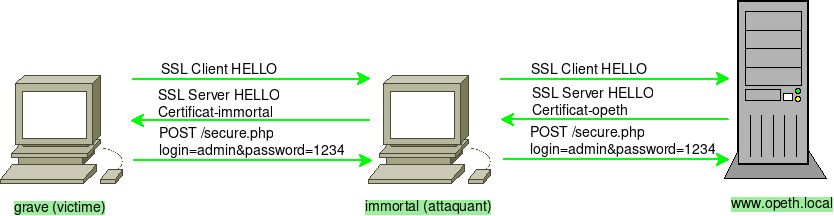
\includegraphics[width=\textwidth]{../medias/https-interception/attack.png}}
\end{figure}

\section{Description de l'attaque}

La méthode que nous allons voir pour intercepter un traffic https n'est pas vraiment une attaque. Pour être menée à bien, la machine placée en homme du milieu doit avoir installé sa propre authorité de certification, et surtout l'avoir rentrée sur la machine du client, en amont.

C'est une chose qui peut être assez dure à réaliser pour un attaquant, mais il y a des cas où cette situation se trouve. Dans le cadre d'une entreprise, il n'est pas rare que les requêtes http des employés passent par un proxy, pour suivre leur activité. Les responsables n'ont par contre, a priori pas moyen de lire les requêtes https.

C'est en fait au contraire assez simple à réaliser dans la mesure où il est facile de rajouter une authorité de certification à la main dans les navigateurs web de tous les employés.

L'idée de la méthode est d'agir comme un simple proxy https. Lors de la connexion initiale du client vers le site web, la machine placée en homme du milieu va récupérer la requête, et établir elle même une connexion avec le serveur distant. Le proxy n'a plus qu'à établir une connexion avec le client, ce qui ne pose pas de problème car l'authorité de certification est acceptée par le navigateur du client.

\section{Notre attaque}

\subsection{Mise en place de l'environnement}

\subsubsection{Machine grave (147.210.13.2)}

Cette machine utilise l'environnement graphique de la distribution Linux Alpine. Le navigateur firefox est utilisé pour la démonstration.

Au lancement de la machine, il faut configurer l'autorité de certification dans firefox. Se reporter au fichier start.sh

\subsubsection{Machine opeth (www.opeth.local)}

Cette machine héberge un serveur HTTP(s) Nginx sur le port 80 et 443. Le certificat utilisé pour les connexions HTTPS a été généré avec les scripts \path{create-ca.sh} et \path{new-cert.sh} de la façon suivante :

\begin{minted}{bash}
cd CA
./create-ca.sh
./new-cert.sh
\end{minted}

Le serveur héberge deux pages :

  - une page index.php que l'on accéde en HTTP et présentant un formulaire de login.

  - une page secure.php que l'on accéde en HTTPS depuis la page index.php.

\subsubsection{Machine immortal (147.210.12.2 - 147.210.13.1)}

C'est sur cette machine que se trouve le PoC de l'attaque, dans le fichier \path{/mnt/host/attack.sh}.

Cette VM est configurée pour forwarder les paquets entre opeth et grave.

\subsection{Démonstration}

Pour lancer l'environnement de test, il faut lancer la commande suivante (on aura récupéré au préalable le dépôt qemunet) :

\begin{minted}{bash}
./qemunet/qemunet.sh -x -S https-interception
\end{minted}

À partir de là, les trois machines sont lancées.

\subsubsection{Étape 1 : avant l'attaque}

Avant que l'attaque soit lancée, nous pouvons accéder à la page de login de manière sécurisée. La machine immortal n'est pas capable de comprendre la communication entre le client (grave) et le serveur (opeth) :

\begin{figure}[H]
  \caption{Attaque https-interception (avant l'attaque)}
  \fbox{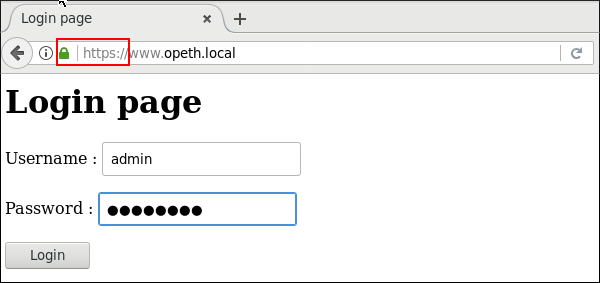
\includegraphics[width=\textwidth]{../medias/https-interception/screen1.png}}
\end{figure}

Ici, on voit que c'est bien le certificat du serveur qui est présenté au navigateur :

\begin{figure}[H]
  \caption{Certificat}
  \fbox{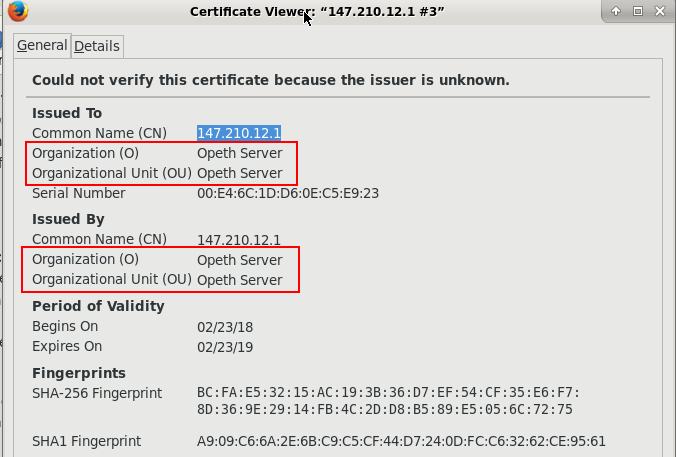
\includegraphics[width=\textwidth]{../medias/https-interception/screen2.png}}
\end{figure}

Nous voici sur la page secure.php, nos données ont transitées de manière chiffrées entre le client et le serveur :

\begin{figure}[H]
  \caption{https se présente normalement}
  \fbox{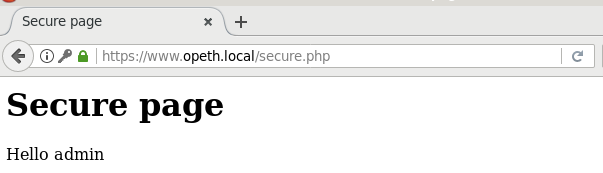
\includegraphics[width=\textwidth]{../medias/https-interception/screen3.png}}
\end{figure}


\subsubsection{Etape 2 : lancement de l'attaque}

Comme expliqué précédement, pour lancer l'attaque, il faut exécuter le fichier \path{/mnt/host/attack.sh} depuis immortal. Voici son contenu :

\begin{minted}{bash}
PROXY_PORT=4242

iptables -t nat -F
iptables -t nat -A PREROUTING -d 147.210.12.1 -p tcp --dport 443 -j REDIRECT --to-port $PROXY_PORT
/mnt/host/https-interception.py $PROXY_PORT
\end{minted}

On peut constater que les flux TCP à destination du port 443 (HTTPS) sont redirigées vers le port d'écoute du proxy qui est chargé d'analyser et traiter les requêtes.

Sur la machine immortal, nous lançons le script de l'attaque :

\begin{figure}[H]
  \caption{Lancement de l'attaque}
  \fbox{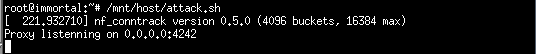
\includegraphics[width=\textwidth]{../medias/https-interception/screen4.png}}
\end{figure}

\paragraph{Explication du code du proxy \\}

Le code du proxy est dans le fichier \path{https-interception.py}. Ce dernier est sensiblement le même que celui utilisé pour l'attaque sslstrip.

\subparagraph{Contexte ssl du proxy \\}

Le proxy doit ajouter son certificat au context pour pouvoir le présenter au client :

\begin{minted}{python}
def __listen(self):
	sock = socket.socket()
	context = ssl.create_default_context(ssl.Purpose.CLIENT_AUTH)
	context.load_cert_chain(certfile=PROXY_CERT, keyfile=PROXY_KEY)
	...
\end{minted}

\subsubsection{Etape 3 : pendant l'attaque}

Lorsque l'attaque est en cours, le certificat présenté au client n'est plus celui d'opeth, mais celui du Proxy, signé par l'autorité de certification. À noter qu'ici si l'autorité de certification du proxy n'avait pas été dans présent dans le navigateur, celui-ci aurait émis une alerte.

Ci-dessous on voit que le certificat présenté est celui du proxy (immortal), et non plus celui du serveur. On voit bien que les empreintes SHA256 sont différentes.

\begin{figure}[H]
  \caption{Le certificat a changé}
  \fbox{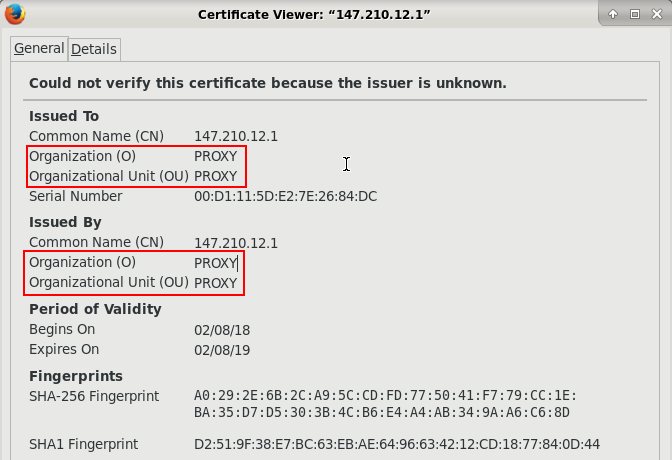
\includegraphics[width=\textwidth]{../medias/https-interception/screen6.png}}
\end{figure}

Si le certificat est accepté par le client et que nous essayons de nous enregistrer :

\begin{figure}[H]
  \caption{Connexion sécurisée}
  \fbox{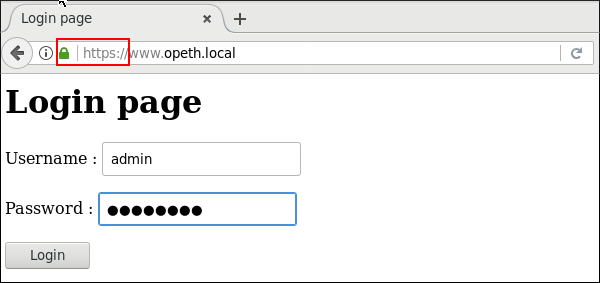
\includegraphics[width=\textwidth]{../medias/https-interception/screen1.png}}
\end{figure}

Nous arrivons bien sur la page secure.php, et notre connection est bien effectuée en HTTPS. Le client n'a constaté aucuns changement au niveau de sa navigation.

\begin{figure}[H]
  \caption{Tout a l'air normal pour le client}
  \fbox{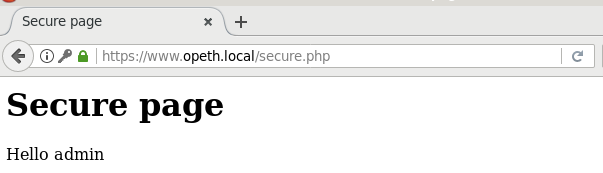
\includegraphics[width=\textwidth]{../medias/https-interception/screen3.png}}
\end{figure}

Par contre, la machine immortal a jouée le rôle d'un proxy et a été capable de récupérer la communication en clair. Ici on voit que le nom d'utilisateur, le mot de passe ainsi que le cookie de session ont pût être capturés :

\begin{figure}[H]
  \caption{L'attaquant a intercepté les informations sensibles}
  \fbox{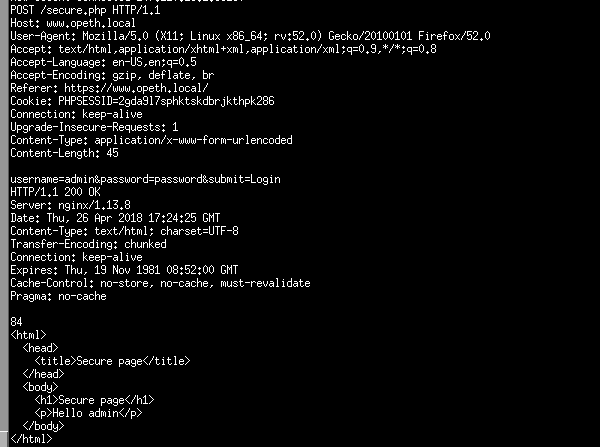
\includegraphics[width=\textwidth]{../medias/https-interception/screen9.png}}
\end{figure}
